\documentclass[a4paper,12pt]{article}

\usepackage[brazilian]{babel}
\usepackage[utf8]{inputenc}
\usepackage[T1]{fontenc}
\frenchspacing
\usepackage{graphicx}
\usepackage{url}

\newcommand\raytracing{\emph{ray tracing}}
\newcommand\Raytracing{\emph{Ray tracing}}

\bibliographystyle{plain}

\title{h3dge: um gerador de imagens 3D em hardware}
\author{Jefferson Chaves Ferreira \\
  \and João Paulo Condé Oliveira Prado \\
  \and Profª Cíntia Borges Margi (orientadora) \\
  \and Pedro Maat Massolino (co-orientador)}

\begin{document}
\maketitle

\section{Introdução}
\subsection{Motivação}
\Raytracing{} é uma técnica utilizada em computação gráfica para sintetizar
imagens 3-D com alto grau de realismo. O método consiste em rastrear a partir de
uma cena pré-definida todos os fenômenos ópticos (reflexões e refrações) a
que são submetidos os raios de luz que chegam ao observador. A figura
\ref{fig:raytraced_glasses} apresenta um exemplo de imagem gerada por esse
algoritmo.

\begin{figure}[htb]
  \centering
  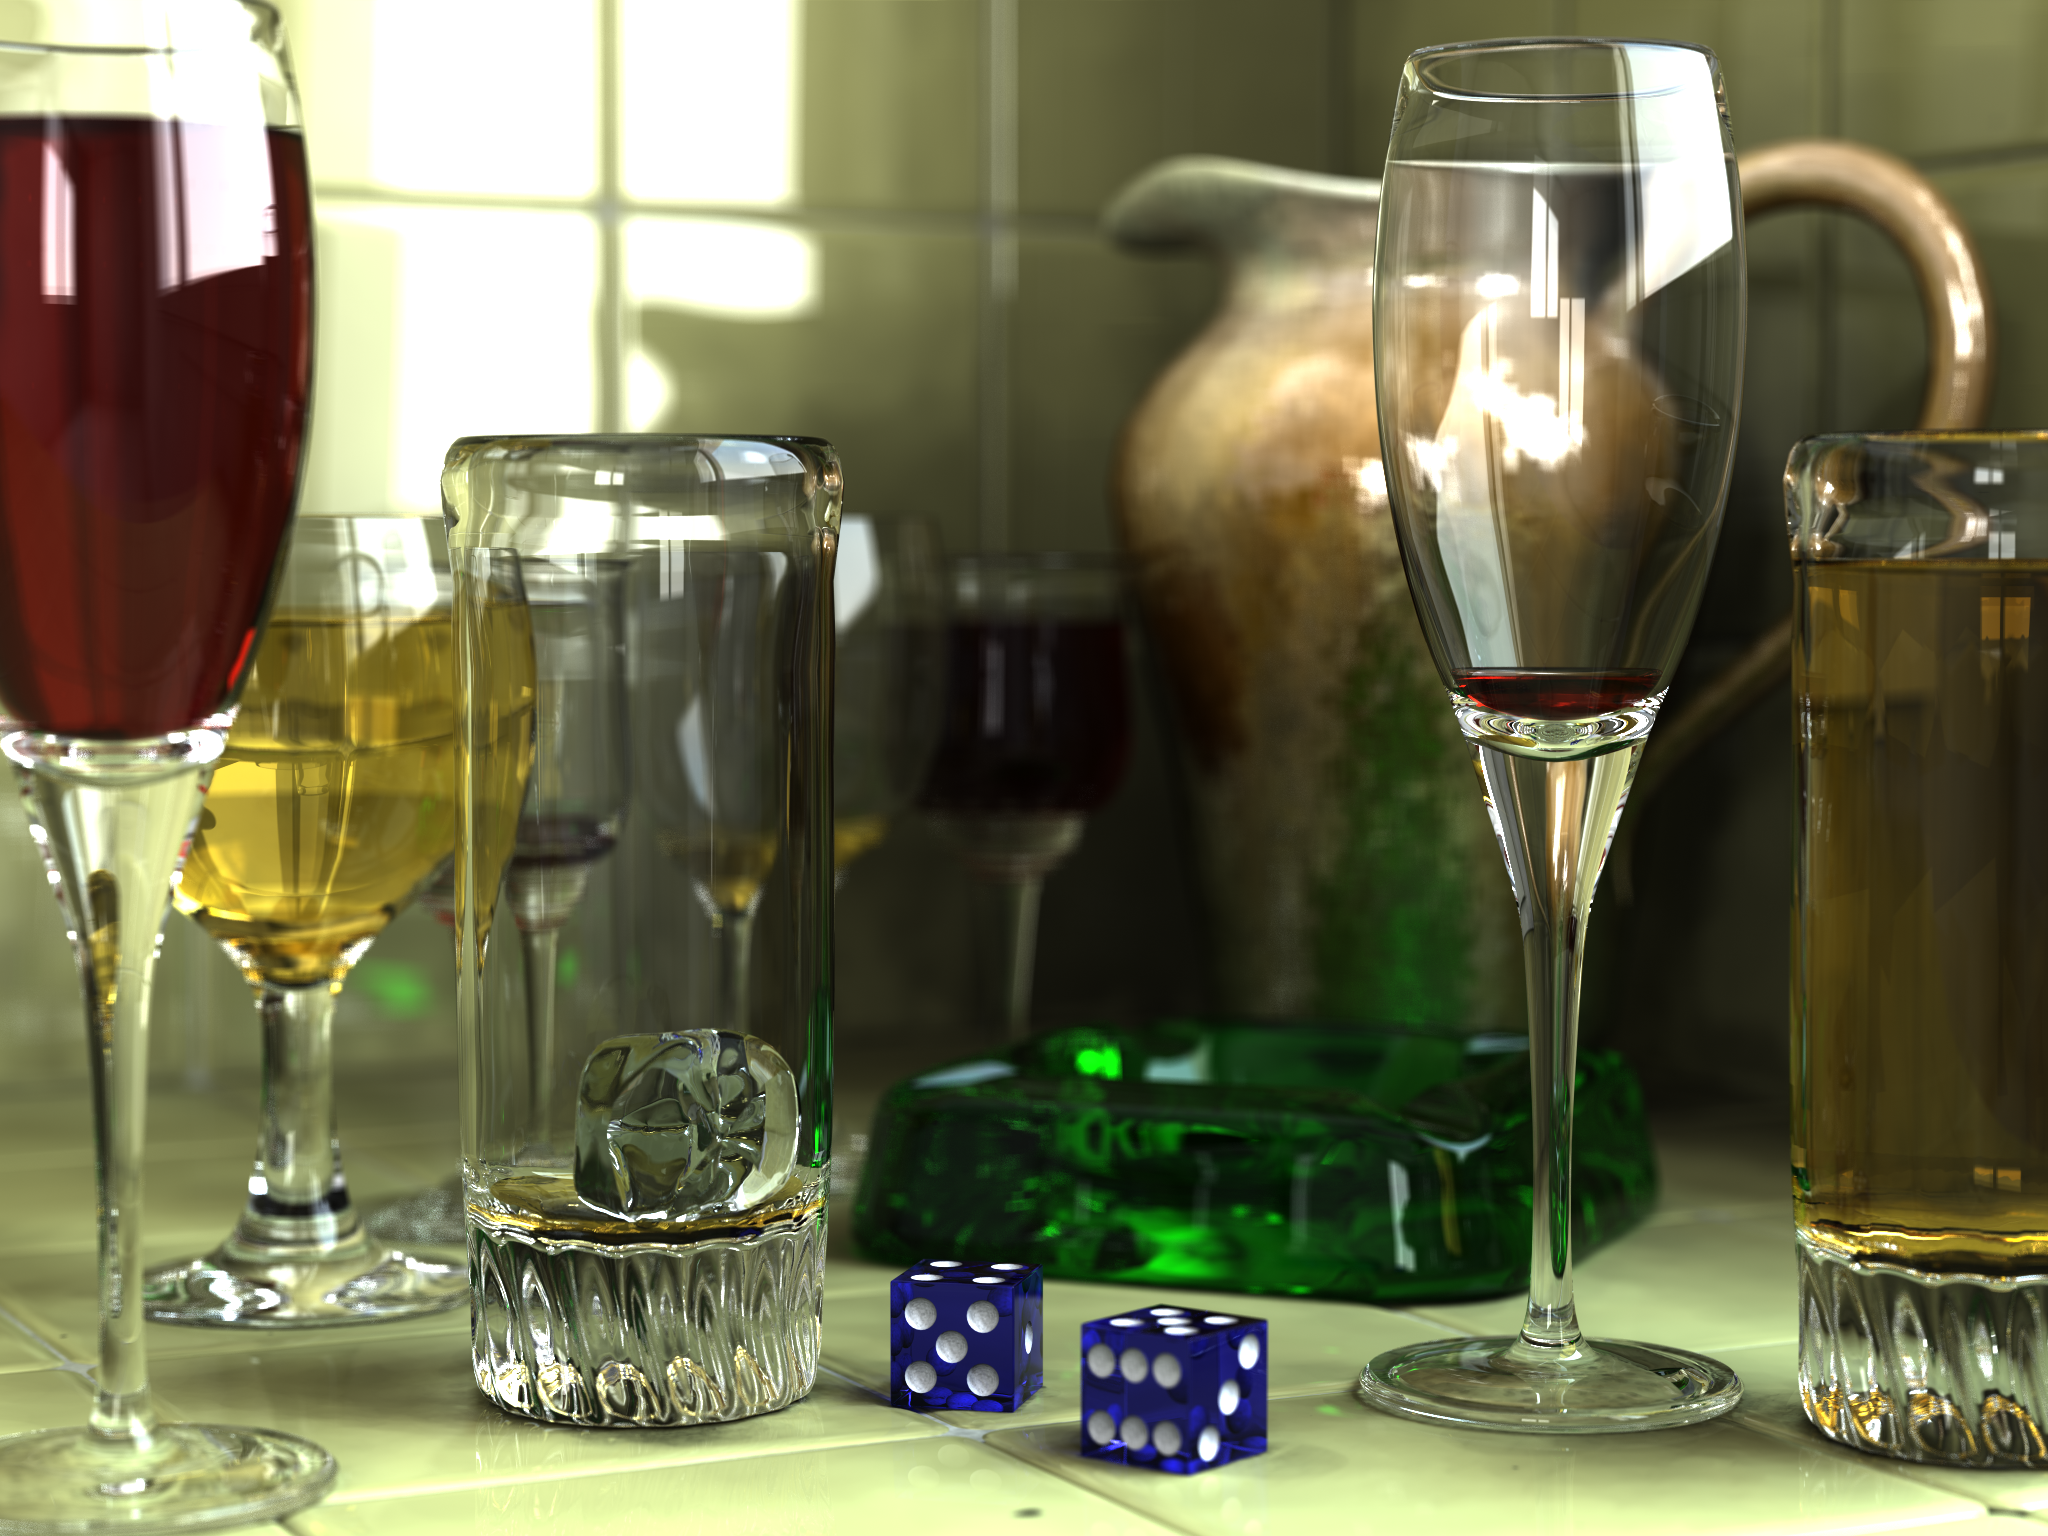
\includegraphics[width=0.75\textwidth]{figures/raytraced_glasses}
  \caption{Exemplo de imagem sintetizada utilizando \raytracing{}. Extraído
    de \cite{wiki:ray_tracing}.}
  \label{fig:raytraced_glasses}
\end{figure}

Embora o princípio subjacente não seja sofisticado, os resultados obtidos por
\raytracing{} são visualmente impressionantes e superiores quando
comparados a imagens geradas por outros algoritmos, como a renderização
\emph{scanline}. Contudo, o \raytracing{} apresenta um alto custo
computacional, sendo indicado para situações onde o tempo de geração das
imagens não é crítico (como fotografias sintetizadas ou efeitos especiais
para filmes e programas de TV); o uso dessa técnica em \emph{video games},
por exemplo, é inviável no estado atual da tecnologia.

\subsection{Trabalhos existentes}

Existem no mercado diversas soluções em software que implementam
a renderização por \raytracing{}, tais como \emph{POV-Ray} e
\emph{mental ray}. No entanto, realizações em hardware são raras e
na maior parte experimentais. Recentemente, a empresa coreana Siliconarts
anunciou o lançamento do primeiro \emph{core} IP para \raytracing{}
\cite{raycore}, o que pode significar o começo da entrada dessa tecnologia
no mercado de consumo em massa.

Atualmente vários centros de pesquisa ao redor do mundo (\cite{hanika} e
\cite{purcell}) trabalham com o objetivo de produzir um protótipo para o uso do
\raytracing{} em tempo real com a finalidade de abrir as portas para o uso desta
tecnologia.

\section{Objetivo}
O objetivo deste trabalho é propor e implementar um raytracer em hardware. O
projeto consiste na definição de uma cena composta de objetos modelados por um
número de triângulos por meio dos quais pode-se obter facilmente a maioria das
figuras em 3D.

Os parâmetros de entrada sao compostos por uma lista de triangulos acompanhados
de suas coordenadas no espaço e das propriedades dos materiais que os compõem
(transparente, opaco, translúcido) e por um número de luzes acompanhadas de
suas propriedades (posiçao no espaço e cor). A partir destas entradas , o
hardware empregará o algoritmo de \raytracing{} e gerará a imagem em 3D com os
efeitos ópticos implementados.

\section{Técnicas}
\subsection{Algoritmo}
\subsubsection{Visão geral}
O princípio de funcionamento do algoritmo é bastante simples: define-se uma
janela de observação sobre a qual a imagem será projetada e posiciona-se o
observador a uma certa distância. Em seguida, para cada pixel da janela
um raio é lançado a partir do observador; calculam-se as interseções
desse raio com os objetos da cena, e para cada interseção são determinados
os raios derivados (refletidos, refratados, etc), que são por sua vez rastreados
da mesma forma, como ilustrado na figura \ref{fig:Ray_trace_diagram}. Enfim, a
cor RGB do pixel é determinada pela composição das contribuições dos raios
calculados.

\begin{figure}[htb]
  \centering
  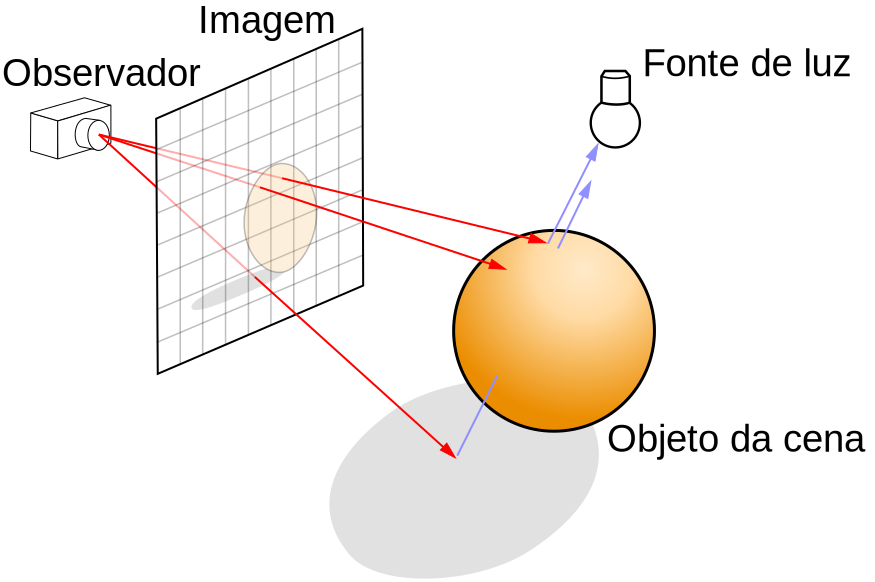
\includegraphics[width=0.75\textwidth]{figures/Ray_trace_diagram}
  \caption{Funcionamento do algoritmo de \raytracing. Adaptado de
    \cite{wiki:ray_tracing}.}
  \label{fig:Ray_trace_diagram}
\end{figure}

As primeiras soluções para ray tracing usaram lógica de ponto flutuante, a qual
requer mais superfície de hardware para sua realizaçao, contudo a utilização de
lógica de ponto fixo permite a elaboraçao de soluções mais eficientes e
robustas. \cite{hanika} Com o objetivo de produzir uma solução robusta, neste
trabalho os cálculos serão feitos empregando-se uma lógica
de ponto fixo com possíveis enquadramentos (mudanças de escala) em cálculos
intermediários.

\subsubsection{Hipóteses simplificadoras}
Em uma primeira abordagem, utilizar-se-ão algumas hipóteses simplificadoras na
implementação do algoritmo de \raytracing:

\begin{itemize}
\item Todos os raios partirão paralelos ao plano de projeção. Tal simplificação
  permite a obtenção de imagens sem implementar um modelo de câmera;
\item Apenas os fenômenos de reflexão e refração serão considerados. Efeitos
  mais complexos, tais como dispersão e aberração cromática, não serão
  implementados;
\item Cada raio partindo do plano de projeção só poderá receber até cinco
  reflexões/refrações. Essa medida é essencial para limitar os
  recursos utilizados.
\end{itemize}

\subsubsection{Entradas e saídas}
O algoritmo de \raytracing{} necessita das seguintes entradas:

\begin{itemize}
\item O tamanho da janela de observação (largura e altura);
\item Os tipos de materiais presentes na cena, definidos por suas
  características físicas (cor, coefficiente de reflexão, de transmissão e
  índice de refração);
\item A cor e a posição de cada uma das fontes de luz;
\item Os triângulos que modelam a cena, definidos por seus respectivos materiais
  e posições de seus vértices.
\end{itemize}

Tais informações podem ser obtidas por meio de arquivos de formato padronizado,
tais como os arquivos \verb|.off| (\emph{Object File Format}, definido em
\cite{Shilane:2004:TPS}), utilizados para representar a geometria de um modelo
com base em polígonos.

A saída do algoritmo é uma sequência de valores RGB correspondentes a cada um
dos pixels da imagem calculada.

\subsubsection{Lançamento de raios}
No nível mais alto de abstração, o algoritmo pode ser visto da seguinte forma:

\begin{footnotesize}
\begin{verbatim}
Para cada pixel da tela:
  Gerar um raio que partirá do pixel atual com direção perpendicular à tela
  Chamar a função de ray tracing com o raio atual e a cena como parâmetros
  Calcular a cor do pixel atual
  Passar ao pixel seguinte
\end{verbatim}
\end{footnotesize}

A função de \raytracing{} é a responsável por encontrar a interseção dos
raios com a cena e calcular as reflexões e refrações. Para evitar um algoritmo
recursivo, que não poderia ser diretamente sintetizado, utiliza-se uma estrutura
arborescente para armazenar os raios secundários.

Cada nó representa um raio e tem no máximo dois filhos: o raio refletido
(esquerdo) e o raio refratado (direito). A árvore é construída em
\emph{pré-ordem}: parte-se do raio principal e calculam-se todos os
raios refletidos; em seguida, calculam-se os raios refratados e para cada raio
criado é repetido o processo de verificação de reflexões e refrações. Tal
mecanismo é ilustrado pela figura \ref{fig:ray_tree}.

\begin{figure}[htb]
  \centering
  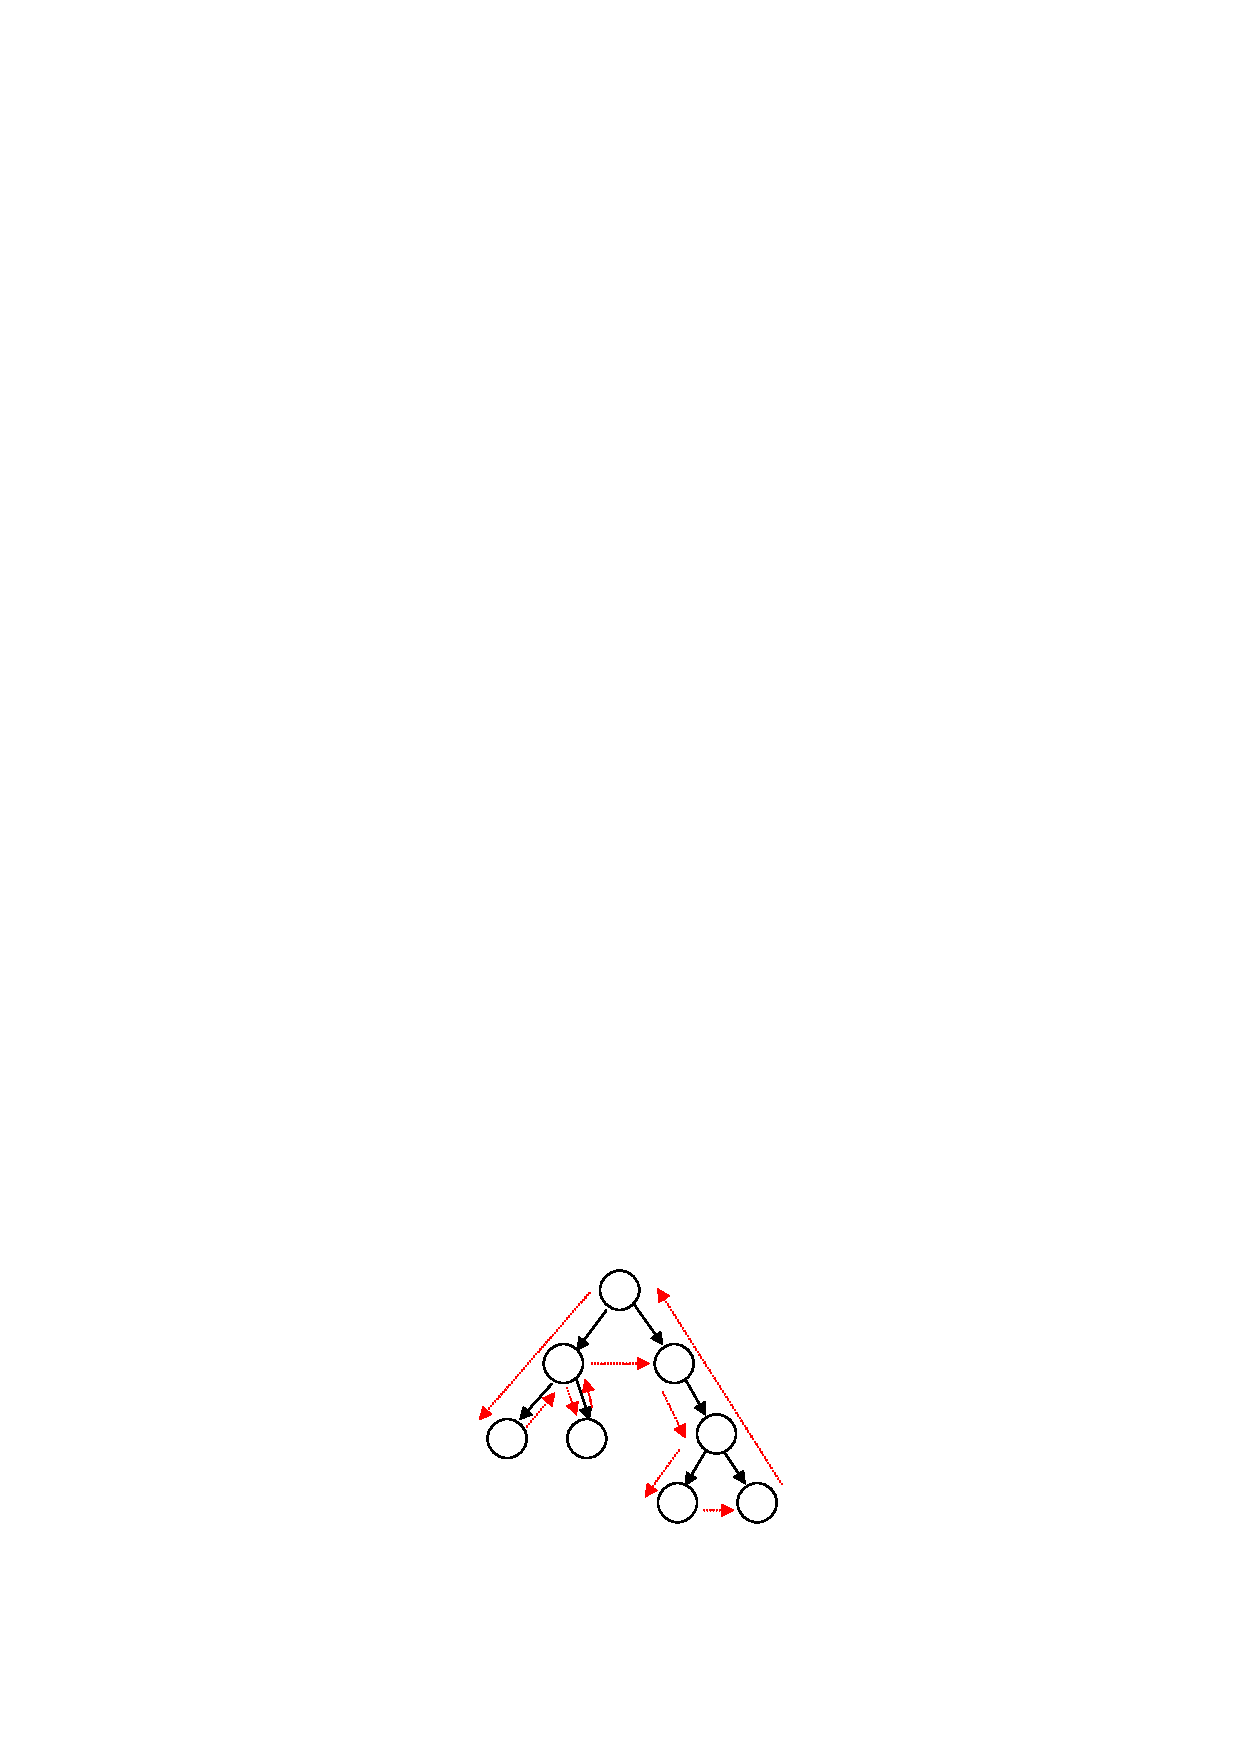
\includegraphics[width=0.5\textwidth]{figures/ray_tree}
  \caption{Criação da árvore de raios refletidos e refratados. As flechas
    vermelhas indicam a sequência do percurso.}
  \label{fig:ray_tree}
\end{figure}

De acordo com as hipóteses simplificadoras estabelecidas, a árvore de raios
nunca terá altura maior do que cinco, haja vista a limitação do número
de reflexões e refrações.

\subsubsection{Otimização com uma árvore $k$-d}
A imagem 3D é gerada a partir da verificaçao da interseção dos raios de luz
incidentes, refletidos e refratados no conjunto de triângulos da cena, contudo,
o processo de verificação tende a ser bem custoso se o algritmo percorrer toda a
lista de triangulos toda vez que a verificaçao de interseção de um raio com um
triangulo for necessária. Para evitar isto, utiliza-se um processo de indexação
espacial por meio de árvores $k$-d que organiza os dados com o objetivo de
percorrer um número mínimo de triangulos e verificar a ocorrencia da interseção
destes triangulos com um raio. Para isto o algoritmo heurístico de área de
superfície descrito por Havran \cite{havran} (capítulo 4) será empregado. A
seguir um pseudo código-fonte de tal algoritmo:

\begin{footnotesize}
\begin{verbatim}
faça
    faça
        se a profundidade máxima nao for atingida
        dividir o eixo do espaço indexável que possui o maior tamanho
        calcular o custo de todos as possiveis posiçoes de corte
        escolher a posição de menor custo
        se o custo for menor que o custo da divisão anterior
            executar a divisao
            criar dois novos nós para armazenar os triângulos compreendidos \
               na parte esquerda e na parte direita da divisão
        senao
            sair do laço
enquanto há nós filhos para serem tratados
\end{verbatim}
\end{footnotesize}

O custo da divisão é calculado da seguinte forma:

\begin{small}
\[
C = \frac{1}{SA(N_{curr})} [ SA(LCN_{curr})(Trig_{left} + Trig_{both})
  + SA(RCN_{curr})(Trig_{right} + Trig_{both}) ]
\]
\end{small}

onde:

\begin{description}
\item[$SA(N_{curr})$] área do nó atual
\item[$SA(LCN_{curr})$] área do candidato a filho esquerdo do nó atual
\item[$SA(RCN_{curr})$] área do candidato a filho direito do nó atual
\item[$Trig_{left}$] número de triângulos à esquerda do valor candidato a
  divisão
\item[$Trig_{right}$] número de triângulos à direita do valor candidato a
  divisão
\item[$Trig_{both}$] número de triângulos que pertencem aos dois lados
  da possível divisão
\end{description}

\subsubsection{Cálculos de interseção}
Uma vez estabelecida a árvore $k$-d de indexação do espaço, as interseções
de um raio com os triângulos da cena podem ser calculadas da seguinte forma:

\begin{footnotesize}
\begin{verbatim}
Calcular a primeira interseção do raio primário com o cubo limitante da cena
Percorrer a árvore k-d e encontrar o primeiro pacote de triângulos \
  correspondente a essa interseção
Enquanto o raio não sair do espaço indexado:
  Encontrar a primeira interseção do raio com um triângulo do pacote
  Se não existir interseção, calcular o ponto em que o raio deixa o pacote \
    e percorrer a árvore k-d para encontrar o próximo pacote
  Senão, calcular os raios secundários, e analizar cada raio novo de acordo \
    com o mesmo procedimento
\end{verbatim}
\end{footnotesize}

\subsection{Arquitetura}

Com a finalidade de implementar o ray tracing , propõe-se a arquitetura da figura \ref{fig:archi_general}. O processador é responsável por calcular a interseção do raio proveniente da janela de observação com o espaço o qual será indexado por meio da árvore kd e por fazer o gerenciamento de cada coprocessador fonecendo-lhes um raio (utilizado para calcular a intersecçao) e o endereço do primeiro pacote de triângulos. Os coprocessadores são responsáveis pela execução do algoritmo de ray tracing. O algoritmo de raytracing pode ser paralelizdo, pois cada raio de luz pode ser tratado de forma independente.

 Na figura \ref{fig:archi_general} sugere-se o emprego de dois coprocessadores, contudo seu número dependerá das especificações técnicas da FPGA a ser empregada. No coprocessador (estrutura na figura \ref{fig:archi_coproc}) há uma memória local que será utilizada para armazenar dados muito utilizados pelo algoritmo de ray tracing cujas estruturas são especificadas a seguir:

\begin{itemize}
\item Dois nós da árvore kd: um com os dados da raiz e outro com os dados do pacote de triângulos em tratamento
\item O endereço do pacote atual
\item O endereço para guardar a intensidade luminosa
\item Um vetor para estocar os triangulos do pacote em processamento
\item Um vetor para os materiais
\item Um vetor para as luzes
\item Uma árvore binária para estocar a sequência de raios refletidos e refratados
\end{itemize}

\begin{figure}[htbp]
  \centering
  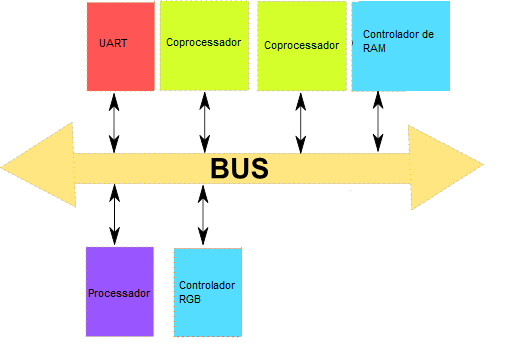
\includegraphics[width=0.95\textwidth]{figures/archi_general}
  \caption{Arquitetura proposta.}
  \label{fig:archi_general}
\end{figure}

\begin{figure}[htbp]
  \centering
  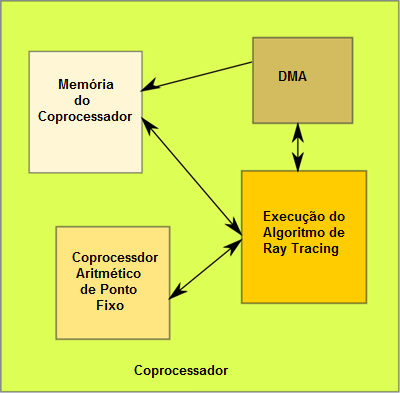
\includegraphics[width=0.5\textwidth]{figures/archi_coproc}
  \caption{Arquitetura do coprocessador.}
  \label{fig:archi_coproc}
\end{figure}

\section{Tarefas}
\subsection{Descrição}
\subsubsection{Especificar formalmente o projeto}
Tarefa materializada neste relatório, corresponde à identificação dos requisitos
do projeto e ao estabelecimento da arquitetura a ser adotada para a
implementação.

\subsubsection{Corrigir e refinar descrição em alto nível}
A descrição atual do raytracer em systemC contém alguns erros. Para a continuação do projeto é necesário identificar e corrigir tais erros que se concentram no algoritmo de busca do pactote mais próximo e na geração da árvore de raios refletidos e refratados.

\subsubsection{Estudo da FPGA}
Em paralelo à correção do modelo em alto nível, estudar-se-ão as possibilidades oferecidas pela FPGA FPGA Xilinx Virtex-5 XC5VFX70T, disponível na Escola Politécnica, para a síntese do projeto.

\subsubsection{Implementar em HDL}
A partir da descrição em alto nível passa-se a descrição em HDL do raytracer. A linguagem de descrição de hardware utilizada será o Verilog.
\subsubsection{Testes}
Com a progressão da descrição dos módulos do raytracer, inicia-se a fase de testes na qual assegura-se o funcionamento correto de todos os módulos implementados.
\subsubsection{Monografia}
O processo de desenvolvimento da monografia acompanhará o avanço do projeto e documentará todas as etapas anteriores.
\subsection{Cronograma}
O cronograma a seguir mostra a disposição temporal de cada uma das etapas anteriores durante o segundo semestre de 2011:

\begin{figure}[h!]
  \centering
  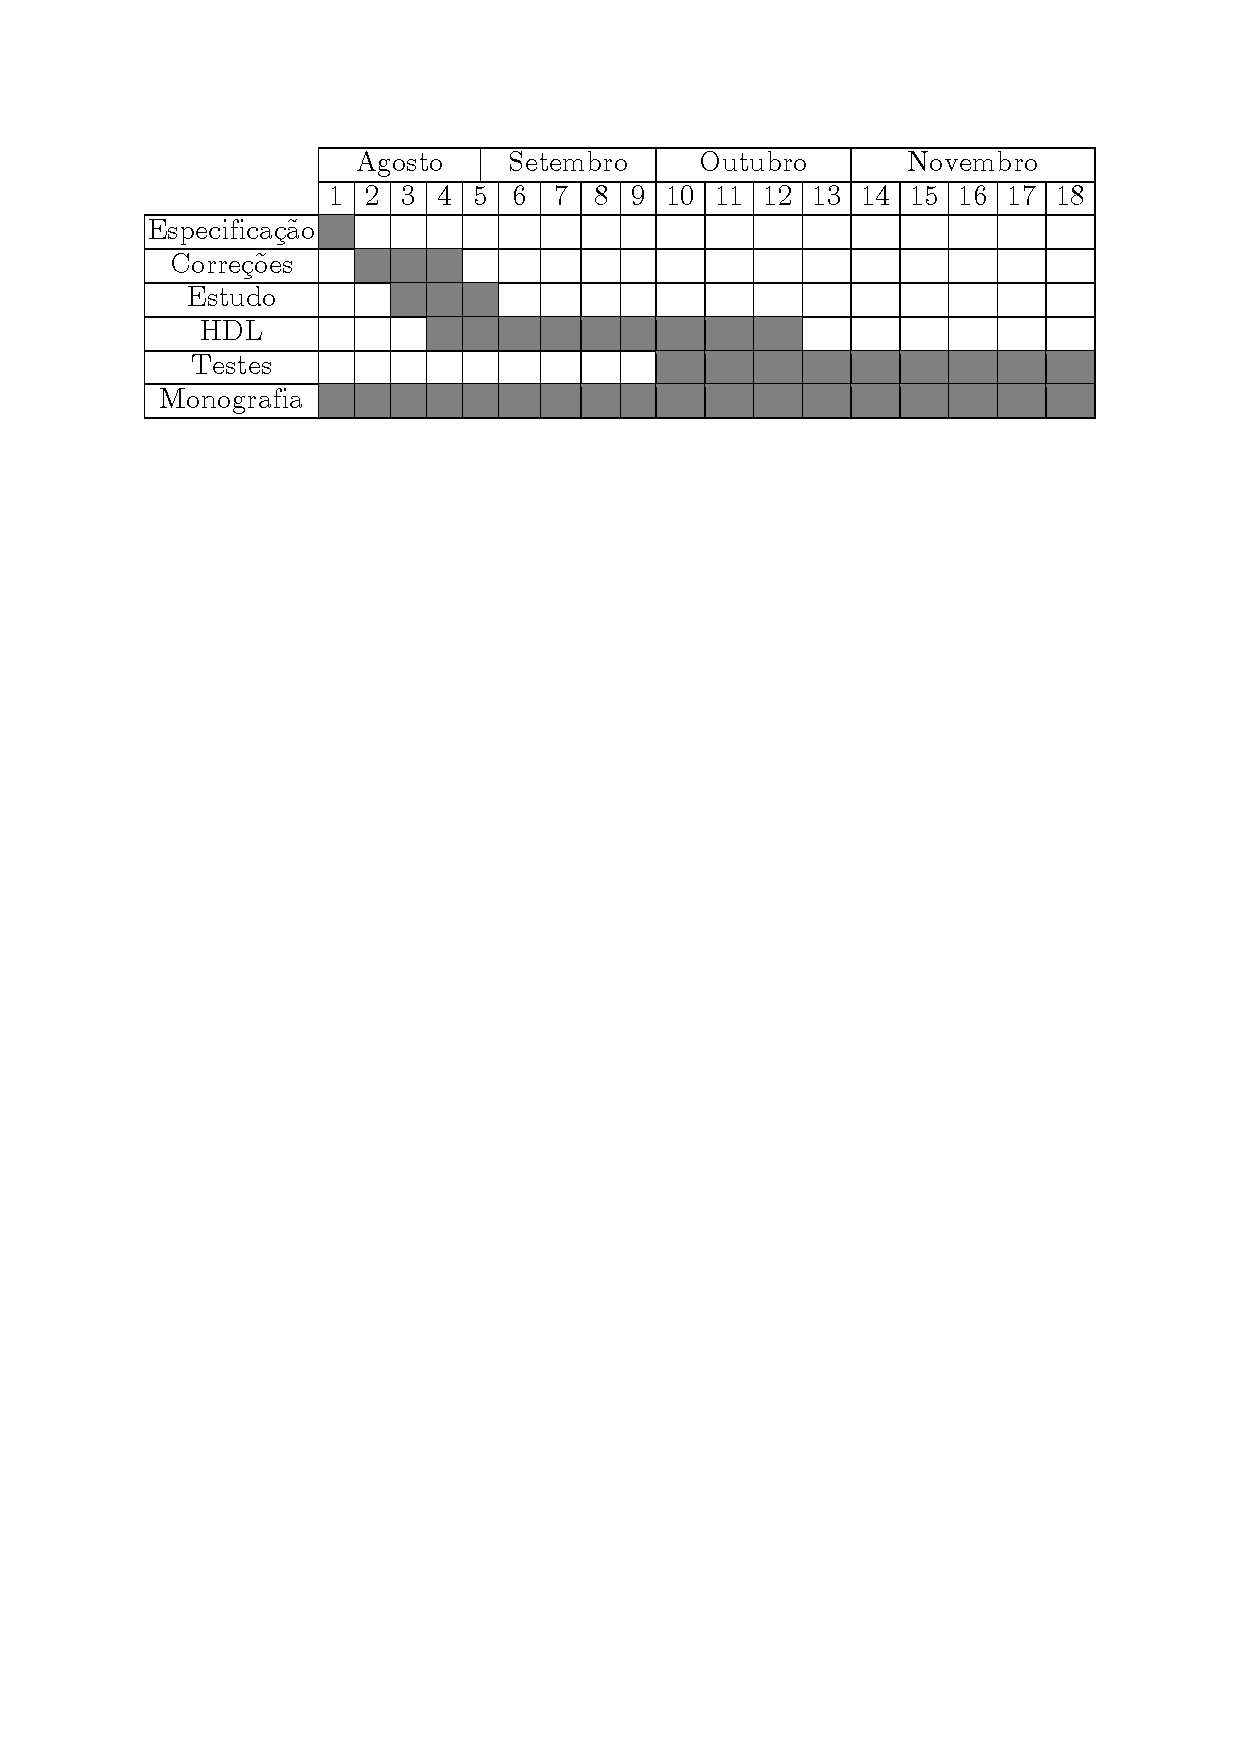
\includegraphics[width=0.95\textwidth]{figures/gantt}
\end{figure}

\newpage

\bibliography{specification}

\end{document}
